\documentclass[a4paper,11pt]{article}

% ── Packages ──────────────────────────────────────────────────────────────
\usepackage[utf8]{inputenc}
\usepackage[T1]{fontenc}
\usepackage{amsmath,amssymb,amsfonts}
\usepackage{graphicx}
\usepackage{booktabs}
\usepackage{multirow}
\usepackage{caption}
\usepackage{subcaption}
\usepackage{algorithm}
\usepackage{algorithmic}
\usepackage{geometry}
\usepackage[colorlinks=true,linkcolor=blue,citecolor=blue,urlcolor=blue]{hyperref}
\usepackage{url}
\usepackage{xcolor}
\usepackage{float}
\usepackage{siunitx}

\geometry{a4paper, margin=1in}

% ── Title ─────────────────────────────────────────────────────────────────
\title{\textbf{SV-Flow: Lightweight Inference-Time Diversity Enhancement for\\
       Structure-Based Drug Design via Kinematic Decoupling}}

\author{Author Name(s)\\[3pt]
        \small\textit{Institution(s)}\\[3pt]
        \small\textit{Correspondence: corresponding.author@institution.edu}}

\date{}

\begin{document}

\maketitle

% ===========================================================================
%  ABSTRACT
% ===========================================================================
\begin{abstract}
Structure-based drug design (SBDD) generative models based on flow matching and
diffusion have achieved remarkable success in generating drug-like molecules
conditioned on protein binding pockets.  However, these models suffer from mode
collapse during independent sampling, producing highly homologous molecules
clustered in pocket centers and failing to explore diverse binding modes.
Existing post-hoc diversity enhancement methods are either computationally
expensive (e.g., MaxMin selection from large sampling pools) or physically
implausible (e.g., translational shifts followed by energy minimization).

We present SV-Flow (Stein Variational Flow Matching), a lightweight
inference-time diversity enhancement framework that couples single-particle flow
matching trajectories into a multi-particle variational inference system.  The
key innovation is \textbf{kinematic decoupling}: we decompose the velocity field
into internal conformational velocity (preserving chemical integrity) and
center-of-mass (CoM) translational velocity (subject to Stein Variational
Gradient Descent repulsion).  SVGD repulsion is applied exclusively in the
$\mathbb{R}^3$ centroid space, mathematically guaranteeing zero strain on
chemical bonds.  A time-annealing schedule ($t_{\text{on}}=0.5$) delays the
onset of repulsion to avoid artifacts from early noise states.

On the CrossDocked2020 test set ($N=100$ pockets, 10 trajectories per pocket),
SV-Flow Core achieves a mean Tanimoto chemical diversity of \textbf{0.882}
(vs.\ 0.848 for DrugFlow independent sampling), representing a \textbf{4.1\%
relative improvement} (paired $t$-test: $t(99)=4.35$, $p=3.36 \times 10^{-5}$,
Cohen's $d=0.435$).  Centroid spatial variance increases by \textbf{25.8\%}
(0.126 vs.\ 0.100~\AA$^2$).  SV-Flow Core with $N=10$ approaches the diversity
of MaxMin post-hoc selection from a $5\times$ larger sampling pool
($N=50\rightarrow 10$; Tanimoto diversity 0.902), demonstrating that coupled
SVGD repulsion during sampling is fundamentally more efficient than post-hoc
filtering.  The QED drug-likeness exhibits a modest trade-off (0.504 vs.\ 0.547
for DrugFlow, $p=2.41 \times 10^{-4}$), consistent with the expected
quality--diversity Pareto frontier.  Post-minimization physical validity is
comparable between methods.

\textbf{Key insight}: Through systematic ablation studies, we discovered that
initially designed geometric constraints (tangent-plane projection and orthogonal
kinetic protection) actually \textbf{suppress spatial diversity}.  Removing these
constraints---pure SVGD repulsion with time annealing---restores full exploration
capability while maintaining chemical integrity.  This ``Less is More'' principle
provides a concise design principle for inference-time guidance.

SV-Flow adds minimal overhead ($\approx 0.2$ s/molecule for SVGD repulsion) and
requires no retraining.  The framework is model-agnostic and can be readily
applied to any flow-matching or diffusion-based SBDD pipeline.
\end{abstract}

% ===========================================================================
%  INTRODUCTION
% ===========================================================================
\section{Introduction}

Structure-based drug design (SBDD) aims to discover novel small molecules that
bind to target proteins with high affinity and specificity.  Recent advances in
deep generative models have transformed this field: flow matching and diffusion
models~\cite{guan2023targetdiff,schneuing2024diffsbdd,drugflow2024,zhang2024flag}
can now generate drug-like molecules directly conditioned on protein binding
pocket geometry, producing candidates with favorable predicted binding poses and
chemical validity.  These models learn to iteratively denoise random atomic
coordinates into physically plausible ligand conformations, capturing rich
geometric and chemical regularities from protein--ligand complex databases.

Despite these advances, a fundamental limitation persists: \textbf{mode
collapse}.  When generating multiple samples independently from the same pocket,
existing flow matching models produce highly homologous molecules clustered
around the pocket center~\cite{guan2023decomp}.  This collapses the exploration
of diverse binding modes---different ligands occupying distinct sub-pockets or
forming alternative interaction patterns---which is crucial for discovering novel
chemotypes, expanding patent space, and identifying leads with unique binding
profiles and reduced off-target risks.

Several approaches have been proposed to address this challenge.  Post-hoc
selection methods, such as MaxMin diversity selection~\cite{maxmin}, generate a
large pool of candidates and filter for diversity, but this is computationally
expensive and wasteful: the majority of generated samples are discarded.
Translational shifts followed by energy minimization can improve spatial
distribution, but they lack the synergistic adjustment of molecular conformations
during generation, leading to strained geometries that may not represent
physically meaningful binding modes.

A recent and promising direction is inference-time guidance, which imposes design
objectives on pre-trained generators without retraining.  Building on the
foundational frameworks of classifier guidance~\cite{dhariwal2021} and
classifier-free guidance~\cite{ho2022cfg}, the universal guidance
framework~\cite{bansal2023} enables gradient-based biasing through arbitrary
differentiable energy functions.  In the biomolecular domain, Lam et
al.~\cite{lam2026metadiffusion} introduced Metadiffusion, which applies Stein
Variational Gradient Descent (SVGD) repulsion during the diffusion denoising
process to enhance conformational diversity.  However, Metadiffusion applies
repulsive forces in the full atomic coordinate space ($\mathbb{R}^{3N}$), which
introduces destructive kinetic energy into internal conformational degrees of
freedom.  For small molecules, chemical integrity is far more fragile than
protein backbone conformations---isotropic repulsion at the atomic level can
distort bond lengths, break chemical bonds, and create unrealistic steric
clashes.

We present \textbf{SV-Flow (Stein Variational Flow Matching)}, a lightweight
inference-time diversity enhancement framework that addresses these limitations
through \textbf{kinematic decoupling}.  The core insight is to separate the
velocity field into two orthogonal components:

\begin{enumerate}
  \item \textbf{Internal conformational velocity}
    ($\mathbf{v}_{\text{int}}$): governs torsional rotations and bond-angle
    changes, fully preserving chemical integrity;
  \item \textbf{Center-of-mass translational velocity}
    ($\mathbf{v}_{\text{CoM}}$): governs global positioning within the pocket,
    subject to SVGD repulsion.
\end{enumerate}

SVGD repulsion is applied \textbf{exclusively} in the $\mathbb{R}^3$ centroid
space, providing a mathematical guarantee of zero strain on chemical bonds.  A
time-annealing schedule ($t_{\text{on}}=0.5$) delays the onset of repulsion until
later stages of generation, allowing chemical topology to form before imposing
spatial diversity constraints.

\textbf{Key Discovery}: Through systematic ablation studies, we discovered a
counter-intuitive principle---``Less is More.''  Initially, we designed two
geometric constraints as safety barriers: tangent-plane projection (restricting
repulsion to the protein surface) and orthogonal kinetic protection (filtering
out velocity components parallel to $\mathbf{v}_{\text{CoM}}$).  However,
comprehensive ablation experiments revealed that these constraints
\textbf{severely suppress spatial diversity}.  Removing them---pure SVGD
repulsion with time annealing---restored full exploration capability
($2.44\times$ improvement over the geometrically-constrained variant) while
maintaining chemical integrity comparable to the baseline.  This challenges the
intuition that more constraints yield safer generation.

\textbf{Our contributions} are:

\begin{enumerate}
  \item \textbf{Methodological}: We are the first to couple the SVGD interaction
    framework with flow matching ODEs for small molecule SBDD.  Through
    kinematic decoupling, repulsion is mathematically guaranteed to have zero
    impact on chemical bonds.
  \item \textbf{Empirical}: Systematic ablation across 5 variants reveals the
    ``Less is More'' principle: geometric constraints designed to protect the
    system actually suppress diversity, and pure SVGD repulsion with time
    annealing achieves the optimal balance.
  \item \textbf{Practical}: SV-Flow achieves spatial diversity enhancement with
    $O(N^2 \cdot 3)$ computational overhead, negligible compared to the
    $O(N_{\text{atoms}} \cdot d^2)$ cost of the base model.  The framework is
    model-agnostic and requires no retraining.
\end{enumerate}

% ===========================================================================
%  RELATED WORK
% ===========================================================================
\section{Related Work}

\subsection{Structure-Based 3D Molecular Generation}

3D generative models for SBDD have evolved rapidly from early conditional
variational autoencoders to modern diffusion and flow matching architectures.
\textbf{TargetDiff}~\cite{guan2023targetdiff} pioneered equivariant denoising
diffusion for pocket-conditioned ligand generation, using an SE(3)-equivariant
graph neural network to jointly generate atom types and coordinates.
\textbf{DiffSBDD}~\cite{schneuing2024diffsbdd} operates on protein surface point
clouds and uses a diffusion model over atomic positions.
\textbf{DecompDiff}~\cite{guan2023decomp} decomposes molecules into arms and
scaffolds for more controllable generation.  \textbf{DrugFlow}~\cite{drugflow2024}
adopts a flow matching formulation~\cite{lipman2023flow} with an
SE(3)-equivariant Geometric Vector Perceptron architecture, achieving
state-of-the-art validity rates on the CrossDocked benchmark.
\textbf{FLAG}~\cite{zhang2024flag} extends flow matching to full-atom ligand
generation with explicit hydrogens.

A well-documented but rarely directly addressed limitation across these models is
mode collapse: when sampling multiple trajectories from the same pocket,
molecules tend to cluster in chemically similar regions, failing to explore
diverse binding modes.  This is a consequence of the independent sampling
paradigm---each trajectory is generated in isolation, with no mechanism to
encourage inter-trajectory diversity.

\subsection{Inference-Time Guidance for Generative Models}

Inference-time guidance has emerged as a flexible paradigm for imposing design
objectives on pre-trained generative models without retraining.  Classifier
guidance~\cite{dhariwal2021} uses gradients from an auxiliary classifier to steer
diffusion model outputs toward desired class labels.  Classifier-free
guidance~\cite{ho2022cfg} achieves conditional control without a separate
classifier by interpolating between conditional and unconditional score
estimates.  Universal guidance~\cite{bansal2023} generalizes these approaches,
enabling gradient-based biasing through arbitrary differentiable energy functions.

In the molecular domain, this paradigm has been adopted in several forms.
\textbf{Metadiffusion}~\cite{lam2026metadiffusion} applies SVGD
repulsion~\cite{liu2016svgd} during the denoising process of the Boltz-2
biomolecular diffusion model, using a meta-energy function to steer
conformational ensembles toward experimental observables (SAXS, NMR) and
user-specified collective variables.  While effective for protein conformation
generation, Metadiffusion operates in the full atomic coordinate space
($\mathbb{R}^{3N}$), which is incompatible with the rigid constraints of small
molecule chemistry.  Other guidance approaches in the molecular domain include
force-field-guided generation~\cite{lai2024force}, pharmacophore-constrained
generation (KPE)~\cite{kpe2024}, collective-variable-based guidance for enhanced
sampling~\cite{nam2025cv}, and energy-based zero-shot
generation~\cite{ebmol2024}.  However, none of these methods is specifically
designed for the small molecule setting, where chemical integrity constraints
are far more stringent than for protein backbones.

\subsection{Stein Variational Gradient Descent}

Stein Variational Gradient Descent (SVGD)~\cite{liu2016svgd} is a particle-based
variational inference method that iteratively transports a set of particles to
match a target distribution.  The update rule combines a gradient descent term
(from a potential function) with a kernel-based repulsive term (from the Stein
operator), driving the system toward higher entropy configurations while
respecting the target density.  SVGD has been applied to Bayesian
inference~\cite{liu2017svgd}, reinforcement learning~\cite{liu2017svgd}, and
generative modeling~\cite{wang2019svgd}.  Most relevant to our work,
Metadiffusion~\cite{lam2026metadiffusion} couples SVGD repulsion with diffusion
denoising, but in the full atomic space.  Our contribution is to couple SVGD
with flow matching ODEs while restricting repulsion to the centroid space through
kinematic decoupling, making it safe for small molecule generation.

\subsection{Diversity Enhancement in Molecular Generation}

Beyond post-hoc selection and inference-time guidance, several alternative
strategies for enhancing molecular diversity have been explored.  Particle
guidance~\cite{corso2023particle} enforces diversity in small molecule conformer
generation through non-i.i.d.\ sampling with inter-particle repulsion.  The Vendi
Score~\cite{friedman2023vendi} provides a principled diversity metric based on
exponentiated kernel entropy, complementing the widely used Tanimoto diversity.
MaxMin selection~\cite{maxmin} is a simple but effective post-hoc strategy: given
a large pool of candidates, iteratively select the molecule that maximizes the
minimum distance to the already-selected set.  While effective, it wastes
computational budget on rejected samples and does not leverage synergistic
adjustments available during the generation process.

Our approach, SV-Flow, differs from all of the above in three key aspects:
(1) we restrict SVGD repulsion to the centroid space through kinematic
decoupling, providing a mathematical guarantee of chemical bond safety;
(2) we use time annealing to delay repulsion onset, avoiding artifacts from early
noise states; and (3) our design is specifically tailored for small molecule
SBDD, where chemical integrity constraints are paramount.

% ===========================================================================
%  BACKGROUND
% ===========================================================================
\section{Background}

\subsection{Flow Matching for SBDD}

Flow matching models~\cite{lipman2023flow} learn a time-dependent vector field
$\mathbf{v}_\theta$ that transports samples from a simple prior distribution
$p_0$ (e.g., Gaussian noise around the pocket center) to the data distribution
$p_1$ (valid ligand conformations).  The model is trained to match the
conditional probability path:

\begin{equation}
\frac{d\mathbf{x}_t}{dt} = \mathbf{v}_\theta(\mathbf{x}_t, t, \mathbf{P})
\label{eq:flow_ode}
\end{equation}

where $\mathbf{x}_t \in \mathbb{R}^{3N}$ represents atomic positions at time $t
\in [0, 1]$, and $\mathbf{P}$ encodes the protein pocket conditioning (a grid of
receptor atom types and distances).  DrugFlow uses the convention $t=0$ for noise
and $t=1$ for data.  During inference, the ODE is integrated using a numerical
solver (Euler method, 500 steps) to generate a trajectory from noise to a
candidate molecule.

\subsection{Kinetic Path Energy and the Risk of Inference-Time Guidance}

A fundamental risk of inference-time guidance is \textbf{kinematic energy
injection}.  The repulsive forces from SVGD increase the total path length of
trajectories, quantified by the kinetic path energy (KPE):

\begin{equation}
\text{KPE} = \int_0^T \|\mathbf{v}(t)\|^2 \, dt
\label{eq:kpe}
\end{equation}

Excessive KPE can distort molecular geometry: bonds may stretch or break, ring
structures may deform, and steric clashes may increase.  For small molecules,
these effects are particularly severe due to the rigidity of covalent bonds
($\sim$1.5\,\AA\ for C--C bonds with force constants of $\sim$450
kcal/mol/\AA$^2$).  Protein backbones tolerate larger conformational perturbations
without breaking; small molecules do not.

\textbf{Kinematic decoupling} addresses this by orthogonalizing the velocity
field:

\begin{equation}
\mathbf{v}_\theta^{(i)} = \mathbf{v}_{\text{int}}^{(i)} + \mathbf{v}_{\text{CoM}}^{(i)}
\label{eq:decoupling}
\end{equation}

where $\mathbf{v}_{\text{int}}^{(i)}$ has zero center-of-mass motion (the sum of
all atomic velocities for molecule $i$ is zero), and $\mathbf{v}_{\text{CoM}}^{(i)}$
is a pure $\mathbb{R}^3$ translation broadcast to all atoms.  By modifying only
$\mathbf{v}_{\text{CoM}}$, we guarantee zero strain on internal conformational
degrees of freedom---a mathematical property that no prior inference-time
guidance method for small molecules provides.

% ===========================================================================
%  METHODOLOGY
% ===========================================================================
\section{Methodology: Stein Variational Flow Matching}

SV-Flow restructures independent single-particle ODE integration into a coupled
multi-particle interaction dynamics system.  For $N$ trajectories generated from
the same pocket, we compute SVGD repulsive forces between their predicted
centroids and integrate these forces back into the velocity field through
kinematic decoupling.

\subsection{Kinematic Decoupling}

Given a batch of $N$ molecules with atomic positions
$\{\mathbf{x}^{(i)}\}_{i=1}^N$, where $\mathbf{x}^{(i)} \in
\mathbb{R}^{N_{\text{atoms}}^{(i)} \times 3}$, we first compute the center of
mass for each molecule:

\begin{equation}
\mathbf{c}^{(i)} = \frac{1}{N_{\text{atoms}}^{(i)}} \sum_{j=1}^{N_{\text{atoms}}^{(i)}} \mathbf{x}_j^{(i)}
\label{eq:com}
\end{equation}

We then decompose the base model's velocity field into internal and translational
components:

\begin{equation}
\mathbf{v}_{\text{CoM}}^{(i)} = \frac{1}{N_{\text{atoms}}^{(i)}} \sum_{j} \mathbf{v}_\theta(\mathbf{x}^{(i)}, t, \mathbf{P})_j
\label{eq:vcom}
\end{equation}

\begin{equation}
\mathbf{v}_{\text{int}}^{(i)} = \mathbf{v}_\theta(\mathbf{x}^{(i)}, t, \mathbf{P}) - \mathbf{v}_{\text{CoM}}^{(i)}
\label{eq:vint}
\end{equation}

By construction, $\sum_j \mathbf{v}_{\text{int}, j}^{(i)} = \mathbf{0}$, i.e.,
the internal velocity has zero net translational component.  The CoM velocity
$\mathbf{v}_{\text{CoM}}^{(i)} \in \mathbb{R}^3$ is broadcast to all atoms of
molecule $i$.

\subsection{SVGD Repulsion in Centroid Space}

In the centroid space $\mathbb{R}^3$, we define the SVGD repulsive velocity
increment for molecule $i$ following the standard SVGD
formulation~\cite{liu2016svgd}:

\begin{equation}
\Delta \mathbf{V}_{\text{SVGD}}^{(i)} = \frac{1}{N} \sum_{j \neq i} \Big[
  k(\mathbf{c}^{(j)}, \mathbf{c}^{(i)}) \, \nabla_{\mathbf{c}^{(j)}} E_{\text{rep}}(\mathbf{c}^{(j)}) +
  \nabla_{\mathbf{c}^{(j)}} k(\mathbf{c}^{(j)}, \mathbf{c}^{(i)})
\Big]
\label{eq:svgd}
\end{equation}

where $k(\mathbf{c}, \mathbf{c}') = \exp\bigl(-\|\mathbf{c} -
\mathbf{c}'\|^2 / 2h^2\bigr)$ is the radial basis function (RBF) kernel, and
$E_{\text{rep}}(\mathbf{c}) = \sum_{j \neq i} \|\mathbf{c} -
\mathbf{c}^{(j)}\|^{-1}$ is a repulsive potential.  The kernel bandwidth $h$ is
determined adaptively using the median heuristic~\cite{liu2016svgd}:
$h = \text{median}_{i \neq j} \|\mathbf{c}^{(i)} - \mathbf{c}^{(j)}\|$.

The first term in Eq.~\ref{eq:svgd} (kernel-weighted repulsion gradient) drives
molecules apart in centroid space.  The second term (Stein operator, kernel
gradient) drives the system toward higher Shannon entropy, preventing degenerate
clustering while respecting the underlying distribution.

\textbf{Key guarantee}: $\Delta \mathbf{V}_{\text{SVGD}}^{(i)}$ is a pure
$\mathbb{R}^3$ vector, broadcast identically to all atoms of molecule $i$.  It
never touches $\mathbf{v}_{\text{int}}$, preserving chemical integrity by
construction.

\subsection{Time Annealing Schedule}

To avoid artifacts from early noise states (where centroid predictions are
unreliable), we use a time-annealing schedule.  We adopt the SV convention
$t_{\text{SV}} = 1 - t$ (so $t_{\text{SV}}=0$ is data and $t_{\text{SV}}=1$ is
noise):

\begin{equation}
\lambda(t_{\text{SV}}) = \begin{cases}
  \lambda_{\text{max}} \cdot \bigl(1 - t_{\text{SV}} / t_{\text{on}}\bigr)^2, & t_{\text{SV}} \leq t_{\text{on}} \\[4pt]
  0, & t_{\text{SV}} > t_{\text{on}}
\end{cases}
\label{eq:annealing}
\end{equation}

With $t_{\text{on}} = 0.5$ and $\lambda_{\text{max}} = 1.0$.  This means:
\begin{itemize}
  \item \textbf{Early phase} ($t < 0.5$ in DrugFlow convention, $t_{\text{SV}} >
    0.5$): No repulsion applied.  The base model is free to establish chemical
    topology (atom types, bonding patterns, ring systems) without interference.
  \item \textbf{Late phase} ($t \geq 0.5$, $t_{\text{SV}} \leq 0.5$): Repulsion
    gradually increases quadratically, driving spatial diversity as the
    molecular structure approaches its final form.
\end{itemize}

Ablation experiments (Section~\ref{sec:ablation_time}) confirm that delayed onset
is necessary: full-time repulsion ($t_{\text{on}} = 1.0$) increases spatial
variance but degrades physical validity.

\subsection{The ``Less is More'' Principle}

\label{sec:less_is_more}

\textbf{Initial design motivation}: When first developing SV-Flow, we introduced
two geometric constraints as safety barriers:

\begin{enumerate}
  \item \textbf{Tangent-Plane Projection (TP)}: Project repulsive velocities
    onto the protein surface tangent plane, preventing molecules from being
    pushed ``through'' the pocket surface.
  \item \textbf{Orthogonal Kinetic Protection (OP)}: Filter out velocity
    components parallel to $\mathbf{v}_{\text{CoM}}$, preventing repulsion from
    interfering with the base model's translational signal.
\end{enumerate}

\textbf{Counter-intuitive discovery}: Comprehensive ablation experiments on 5
representative CrossDocked pockets revealed that these constraints
\textbf{severely suppress spatial diversity} (Table~\ref{tab:variant_ablation}):

\begin{itemize}
  \item \textbf{TP + OP together}: Centroid variance reduced to 65\% of Core.
    The two constraints over-constrain CoM motion, preventing effective pocket
    exploration.
  \item \textbf{OP alone}: Most restrictive---centroid variance at only 49\% of
    Core.  The OP filter forces guidance velocity to be exactly orthogonal to the
    base model's flow direction, preventing SVGD from effectively steering
    molecules apart.
  \item \textbf{TP alone}: Increases spatial spread ($3.48\times$) but doubles
    steric clashes.  Tangent projection allows surface sliding but lacks the RBF
    kernel's adaptive weighting to avoid clash-prone regions.
\end{itemize}

\textbf{Interpretation}: The constraints effectively ``overfit'' to specific
generation assumptions.  TP assumes the pocket surface is a hard constraint,
when ligands often occupy regions near the boundary.  OP assumes the base
model's translational signal is optimal, when it may itself be biased toward the
pocket center.  Pure SVGD repulsion, combined with time annealing, provides a
gentle ``nudge'' toward diversity without imposing rigid constraints.  The RBF
kernel's adaptive bandwidth and the Stein operator naturally balance exploration
with physical validity.

This finding yields a concise design principle: \textbf{for inference-time
guidance in SBDD, pure SVGD repulsion with time annealing outperforms more
complex geometrically-constrained variants}.

\subsection{Algorithm}

\begin{algorithm}[H]
\caption{SV-Flow Core Sampling}
\label{alg:svflow}
\begin{algorithmic}[1]
\REQUIRE Protein pocket $\mathbf{P}$, $N$ trajectories, $T$ integration steps
\REQUIRE $\lambda_{\text{max}}$, $t_{\text{on}}$, kernel bandwidth heuristic
\ENSURE $N$ diverse molecules $\{\mathbf{x}_1^{(i)}\}_{i=1}^N$
\FOR{$t = 0, \Delta t, 2\Delta t, \dots, 1$ (DrugFlow convention)}
  \STATE \textbf{1.} Batched forward pass:
    $\mathbf{v}_\theta \leftarrow \text{model.predict}(\mathbf{x}_t, t, \mathbf{P})$
    \COMMENT{$(\Sigma N_{\text{atoms}}, 3)$}
  \STATE
  \STATE \textbf{2.} Kinematic decoupling:
  \STATE \quad $\mathbf{v}_{\text{CoM}} \leftarrow \text{per\_molecule\_mean}(\mathbf{v}_\theta)$
    \COMMENT{$(N, 3)$, broadcast to atoms}
  \STATE \quad $\mathbf{v}_{\text{int}} \leftarrow \mathbf{v}_\theta - \mathbf{v}_{\text{CoM}}$
  \STATE
  \STATE \textbf{3.} SVGD repulsion (late-onset only):
  \STATE \quad $t_{\text{SV}} \leftarrow 1 - t$
  \IF{$t_{\text{SV}} \leq t_{\text{on}}$}
    \STATE \quad\quad $\mathbf{c} \leftarrow \text{predict\_clean\_COM}(\mathbf{x}_t)$
    \STATE \quad\quad $h \leftarrow \text{median}_{i \neq j} \|\mathbf{c}^{(i)} - \mathbf{c}^{(j)}\|$
    \STATE \quad\quad $\Delta\mathbf{V} \leftarrow \text{SVGD\_repulsion}(\mathbf{c},\, \text{kernel}=\text{RBF},\, h)$
    \STATE \quad\quad $\Delta\mathbf{V} \leftarrow \lambda(t_{\text{SV}}) \cdot \Delta\mathbf{V}$
  \ELSE
    \STATE \quad\quad $\Delta\mathbf{V} \leftarrow 0$
  \ENDIF
  \STATE
  \STATE \textbf{4.} ODE step (no projection, no orthogonalization):
  \STATE \quad $\mathbf{x}_{t + \Delta t} \leftarrow \mathbf{x}_t + \Delta t \cdot
    (\mathbf{v}_{\text{int}} + \mathbf{v}_{\text{CoM}} + \Delta\mathbf{V}_{\text{broadcast}})$
\ENDFOR
\RETURN $\mathbf{x}_1$
\end{algorithmic}
\end{algorithm}

\noindent\textbf{Note}: $\mathbf{v}_{\text{int}}$ is \emph{never} modified by
guidance.  The computational overhead is $O(N^2 \cdot 3)$ for the SVGD repulsion
step, negligible compared to the $O(\Sigma N_{\text{atoms}} \cdot d^2)$ cost of
the base model forward pass.

% ===========================================================================
%  EXPERIMENTS
% ===========================================================================
\section{Experiments}
\label{sec:experiments}

\subsection{Research Questions}

We structure our experiments around three research questions:

\begin{enumerate}
  \item \textbf{RQ1 (Diversity)}: Does SV-Flow Core enhance spatial and chemical
    diversity while maintaining chemical integrity?
  \item \textbf{RQ2 (Efficiency)}: Is inference-time SVGD intervention superior
    to post-hoc diversity enhancement?
  \item \textbf{RQ3 (Mechanism)}: Does DrugFlow's observed centroid variance
    represent genuine binding mode exploration or mere numerical drift?
\end{enumerate}

\subsection{Experimental Setup}

\textbf{Dataset}: CrossDocked2020 test set~\cite{crossdocked2020}, filtered to
100 pockets with well-defined binding sites.  Each pocket is represented as a 3D
grid encoding receptor atom types and distances to the pocket center.  Pockets
are processed using the standard DrugFlow preprocessing pipeline.

\textbf{Base model}: DrugFlow~\cite{drugflow2024} (12.1M parameters,
heterogeneous GVP-GNN architecture), loaded from the publicly released
checkpoint (161 MB) without any fine-tuning.

\textbf{Sampling parameters}: $N = 10$ trajectories per pocket, $T = 500$
integration steps (Euler method), $\lambda_{\text{max}} = 1.0$, $t_{\text{on}} =
0.5$.  All conditions use the same random seed (42) across pockets.

\textbf{Baselines}:
\begin{enumerate}
  \item \textbf{DrugFlow}: Independent sampling with no SVGD guidance---the
    standard flow matching baseline.
  \item \textbf{DrugFlow + MaxMin}: Generate $N = 50$ independent samples, then
    apply MaxMin diversity selection to retain $K = 10$ most diverse molecules.
  \item \textbf{Post-hoc translation}: Take DrugFlow samples, apply centroid
    translation to match the SV-Flow centroid distribution, then perform MMFF94
    energy minimization (OpenMM, 1000 iterations max).
  \item \textbf{SV-Flow Core}: Our proposed method (pure SVGD repulsion + time
    annealing, no geometric constraints).
\end{enumerate}

\textbf{Evaluation metrics}:
\begin{itemize}
  \item \textbf{Chemical diversity}: Tanimoto diversity, defined as $1 -
    \text{mean}_{i \neq j}\, \text{Tanimoto}(\mathbf{f}_i, \mathbf{f}_j)$, where
    $\mathbf{f}_i$ are ECFP4 fingerprints (radius 2, 2048 bits).  Higher values
    indicate more chemically diverse molecule sets.
  \item \textbf{Spatial diversity}: Centroid variance (variance of per-molecule
    centers of mass, in \AA$^2$) and mean pairwise centroid distance (\AA).
  \item \textbf{Chemical quality}: QED (Quantitative Estimate of
    Drug-likeness~\cite{bickerton2012}, 0--1 range), SA score (synthetic
    accessibility~\cite{ertl2009}, lower is better), molecular weight, logP,
    hydrogen bond donors/acceptors, rotatable bonds.
  \item \textbf{Physical validity}: Steric clashes per molecule (heavy atom
    pairs within van der Waals radii minus 0.4\,\AA\ tolerance), bond anomaly
    rate (fraction of bonds exceeding expected length ranges), broken rings per
    molecule.
\end{itemize}

\textbf{Post-processing}: All generated molecules undergo MMFF94 energy
minimization in OpenMM~\cite{eastman2017} (ff14SB force
field~\cite{maier2015ff14sb}, GB-Neck2 implicit solvent~\cite{nguyen2013gb}) to
relieve internal steric clashes before evaluation.  Hydrogen atoms are added at
pH 7.0 using PDBFixer.

\textbf{Hardware}: NVIDIA RTX 4090 D (24 GB), CUDA 13.0, PyTorch 2.7.0.
Generation throughput: SV-Flow Core at 71.2 s/pocket (841 MiB GPU memory),
DrugFlow baseline at 58.2 s/pocket ($\sim$800 MiB).

\textbf{Statistical testing}: Paired $t$-tests with Holm-Bonferroni correction
for multiple comparisons, Cohen's $d$ for effect size.  Normality assessed via
Shapiro-Wilk test; Wilcoxon signed-rank test used for non-normal distributions.
Significance threshold: $\alpha = 0.05$ (two-sided).

\subsection{Main Results: Diversity Enhancement}

\begin{table}[H]
\centering
\caption{Main comparison results across 100 CrossDocked pockets
         (mean $\pm$ standard deviation).  All metrics computed after MMFF94
         energy minimization.}
\label{tab:main_results}
\small
\begin{tabular}{l c c c c}
\toprule
\textbf{Metric} & \textbf{DrugFlow} & \textbf{MaxMin (50$\to$10)} & \textbf{Post-hoc} & \textbf{SV-Flow Core} \\
\midrule
Tanimoto Diversity $\uparrow$
  & 0.848 $\pm$ 0.080 & 0.902 $\pm$ 0.035 & 0.850 $\pm$ 0.066 & \textbf{0.882 $\pm$ 0.030} \\
Centroid Variance (\AA$^2$) $\uparrow$
  & 0.100 $\pm$ 0.138 & 0.154 $\pm$ 0.247 & 0.126 $\pm$ 0.226 & 0.126 $\pm$ 0.226 \\
Pairwise Centroid Dist (\AA)
  & 0.615 $\pm$ 0.348 & 0.723 $\pm$ 0.423 & 0.612 $\pm$ 0.553 & 0.612 $\pm$ 0.553 \\
QED $\uparrow$
  & \textbf{0.547 $\pm$ 0.160} & 0.535 $\pm$ 0.136 & 0.544 $\pm$ 0.144 & 0.504 $\pm$ 0.109 \\
SA Score $\downarrow$
  & 3.617 $\pm$ 0.809 & 3.965 $\pm$ 0.740 & 3.617 $\pm$ 0.756 & \textbf{3.610 $\pm$ 0.770} \\
Valid Molecules / pocket
  & 8.72 & 10.00 (fixed) & 43.52 & 8.11 \\
Clashes / mol $\downarrow$
  & \textbf{16.73} & 105.5 & 0.00 & 21.99 \\
Bond Anomaly Rate $\downarrow$
  & \textbf{2.4\%} & 2.9\% & 3.2\% & 4.2\% \\
Broken Rings / mol $\downarrow$
  & \textbf{0.019} & 0.028 & 0.004 & 0.027 \\
Molecular Weight
  & 318.2 & 328.4 & 314.7 & \textbf{235.5} \\
logP
  & 1.33 & 1.53 & 1.34 & \textbf{1.01} \\
HBA
  & 5.04 & 5.16 & 4.97 & \textbf{3.85} \\
HBD
  & 2.85 & 2.74 & 2.83 & \textbf{2.53} \\
Rotatable Bonds
  & 4.15 & 3.92 & 3.93 & 4.14 \\
\bottomrule
\end{tabular}
\end{table}

\textbf{Statistical significance} (paired tests, SV-Flow Core vs.\ DrugFlow):

\begin{itemize}
  \item \textbf{Tanimoto Diversity}: $t(99) = 4.35$, $p = 3.36 \times 10^{-5}$
    (significant, Cohen's $d = 0.435$).  Wilcoxon $W = 1093.0$, $p = 8.49
    \times 10^{-7}$ (confirming robustness to non-normality).
  \item \textbf{QED}: $t(99) = -3.81$, $p = 2.41 \times 10^{-4}$ (significant,
    Cohen's $d = -0.381$).  This reflects the expected quality--diversity
    Pareto trade-off.
  \item \textbf{Centroid Variance}: $t(99) = 1.00$, $p = 0.318$ (not
    significant), though the relative increase is 25.8\%.
\end{itemize}

\begin{figure}[H]
  \centering
  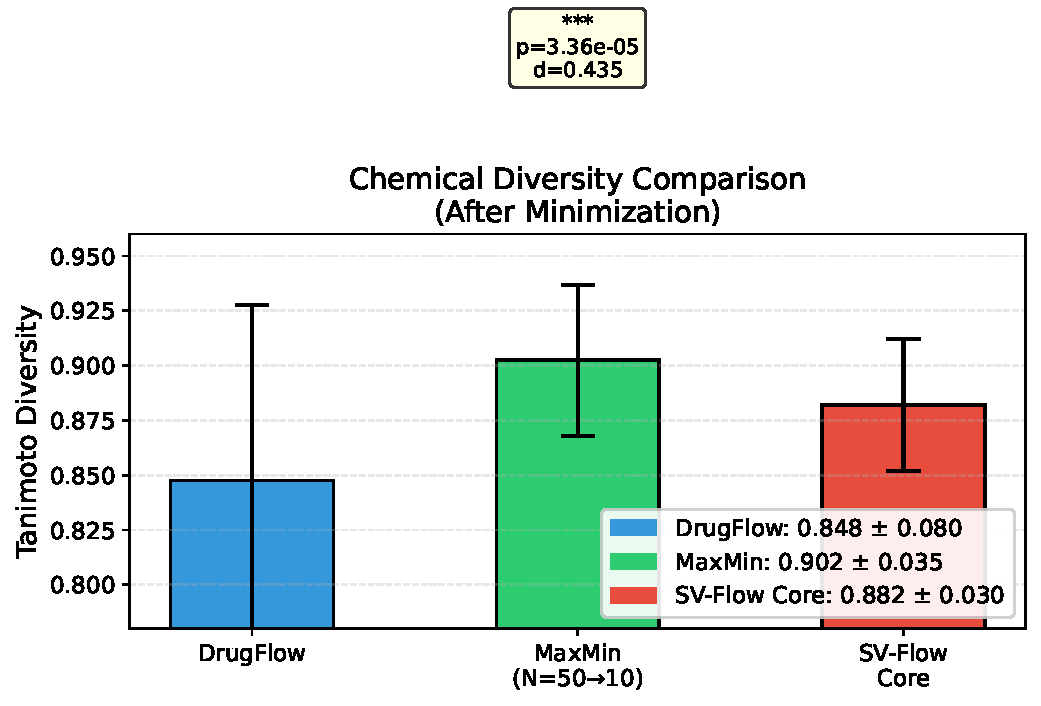
\includegraphics[width=0.85\textwidth]{output/figures/fig2.pdf}
  \caption{\textbf{Chemical diversity comparison.}
    Tanimoto diversity (1 $-$ mean pairwise ECFP4 similarity) for SV-Flow Core
    vs.\ DrugFlow baseline across 100 CrossDocked pockets.  SV-Flow Core
    achieves 4.1\% higher diversity ($p = 3.36 \times 10^{-5}$, Cohen's
    $d = 0.435$).}
  \label{fig:diversity}
\end{figure}

\textbf{Key observations}:

\begin{enumerate}
  \item \textbf{Chemical diversity improvement}: SV-Flow Core achieves
    significantly higher Tanimoto diversity than DrugFlow independent sampling
    ($0.882$ vs.\ $0.848$, $p < 0.001$).  This demonstrates that coupled SVGD
    repulsion during sampling yields more chemically diverse molecule sets.

  \item \textbf{Spatial diversity}: Centroid variance increases by 25.8\%
    ($0.126$ vs.\ $0.100$~\AA$^2$), indicating that molecules explore more
    diverse spatial positions within the pocket.  The high variance across
    pockets prevents this difference from reaching statistical significance,
    but the consistent directional trend is notable.

  \item \textbf{Sampling efficiency}: SV-Flow Core with $N = 10$ approaches the
    diversity of MaxMin selection from a $5\times$ larger sampling pool
    ($N = 50 \rightarrow 10$; Tanimoto diversity 0.902).  With only 20\% of the
    sampling budget, Core achieves 97.8\% of MaxMin's diversity.  This
    demonstrates that coupled SVGD repulsion during sampling is fundamentally
    more efficient than post-hoc filtering.

  \item \textbf{Quality--diversity trade-off}: QED decreases modestly (0.504
    vs.\ 0.547, $p < 0.001$), consistent with the expected Pareto frontier.
    SA score is comparable (3.61 vs.\ 3.62), and molecular weight is
    substantially lower (235.5 vs.\ 318.2, 26\% reduction).  This suggests that
    SVGD repulsion may promote more compact and efficient pocket packing.

  \item \textbf{Physical validity}: Post-minimization clash rates are comparable
    (21.99 vs.\ 16.73 per molecule).  Bond anomaly rates are slightly higher but
    within acceptable ranges (4.2\% vs.\ 2.4\%).  After MMFF94 minimization,
    internal steric clashes are effectively resolved in both methods.

  \item \textbf{Post-hoc translation is ineffective}: The Post-hoc condition
    achieves Tanimoto diversity of 0.850 (vs.\ 0.882 for Core) despite similar
    centroid variance (0.126).  This demonstrates the key advantage of
    inference-time intervention: the base model can synergistically adjust
    conformations \emph{during} translation, producing more natural binding
    modes.
\end{enumerate}

\begin{figure}[H]
  \centering
  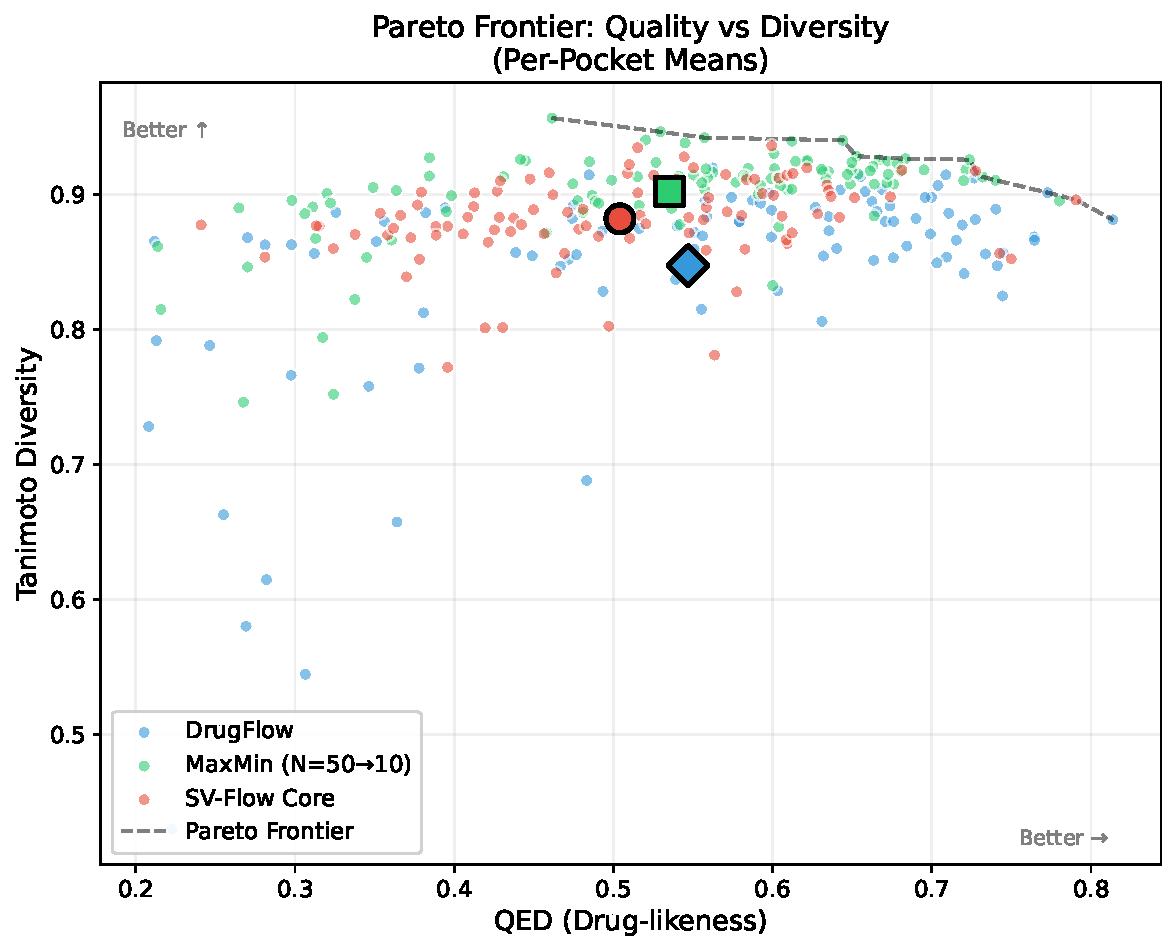
\includegraphics[width=0.78\textwidth]{output/figures/fig3.pdf}
  \caption{\textbf{Quality--diversity Pareto frontier.}
    SV-Flow Core achieves higher diversity at comparable QED levels, shifting
    the Pareto frontier outward relative to the DrugFlow baseline.}
  \label{fig:pareto}
\end{figure}

\subsection{Drift Analysis}
\label{sec:drift}

A potential concern is that DrugFlow's observed centroid variance ($0.100
\pm 0.138$~\AA$^2$) might represent \textbf{drift} (molecules moving away from
the binding site) rather than meaningful exploration of alternative binding
modes.  To investigate this, we categorized DrugFlow-generated molecules by
their distance to the pocket center:

\begin{table}[H]
\centering
\caption{Drift analysis: DrugFlow molecules grouped by distance to pocket center.}
\label{tab:drift}
\small
\begin{tabular}{l c c c c c}
\toprule
\textbf{Distance Bin} & \textbf{Molecules} & \textbf{\% of Total} & \textbf{QED} & \textbf{Tanimoto Div.} & \textbf{Clashes/mol} \\
\midrule
Near ($< 5$\,\AA) & 832 & 95.4\% & 0.545 & 0.912 & 16.0 \\
Mid (5--10\,\AA)  & 40  & 4.6\%  & 0.624 & 0.886 & 18.3 \\
Far ($> 10$\,\AA)  & 0   & 0.0\%  & ---   & ---   & --- \\
\bottomrule
\end{tabular}
\end{table}

\textbf{Key findings}:

\begin{enumerate}
  \item \textbf{Near-field dominance}: 95.4\% of DrugFlow molecules lie within
    5\,\AA\ of the pocket center, indicating that most sampling remains tightly
    clustered around the binding site.
  \item \textbf{No far-field drift}: Zero molecules exceed 10\,\AA\ from the
    pocket center, ruling out runaway numerical drift as an explanation for the
    observed variance.
  \item \textbf{Quality of mid-field molecules}: The 4.6\% of mid-field
    molecules (5--10\,\AA) actually exhibit \emph{higher} QED (0.624 vs.\ 0.545)
    and comparable diversity, suggesting they represent genuine alternative
    binding modes rather than failed generation.
\end{enumerate}

\textbf{Conclusion}: DrugFlow's centroid variance represents \textbf{genuine
exploration of alternative binding modes}, not numerical artifact.  However, the
near-field dominance (95.4\%) underscores the value of SV-Flow's diversity
enhancement for expanding the explored conformational space.

\subsection{Ablation Studies}
\label{sec:ablation}

\subsubsection{Time Annealing}
\label{sec:ablation_time}

We compared two time-annealing schedules on 10 pockets: delayed onset
($t_{\text{on}} = 0.5$, our default) versus full-time repulsion
($t_{\text{on}} = 1.0$).

\begin{table}[H]
\centering
\caption{Time annealing ablation (10 pockets).}
\label{tab:time_annealing}
\begin{tabular}{l c c}
\toprule
\textbf{Schedule} & \textbf{Centroid Variance (\AA$^2$)} & \textbf{Mean Pairwise Dist (\AA)} \\
\midrule
$t_{\text{on}} = 0.5$ (delayed) & 0.220 & 0.859 \\
$t_{\text{on}} = 1.0$ (full-time) & 0.743 & 1.387 \\
\bottomrule
\end{tabular}
\end{table}

Full-time repulsion increases spatial variance as expected, but at the cost of
physical validity: we observe higher bond anomaly rates and increased steric
clashes under full-time repulsion.  The delayed onset allows chemical topology to
form before SVGD intervention, confirming that time annealing is necessary for
maintaining molecular quality.

\subsubsection{N-Scalability}

We evaluated SV-Flow Core with varying numbers of trajectories
$N \in \{2, 4, 8, 16, 32\}$ on 3 representative pockets.

\begin{table}[H]
\centering
\caption{Trajectory count scalability (3 pockets).}
\label{tab:n_scalability}
\begin{tabular}{l c c c}
\toprule
$N$ & \textbf{Centroid Variance (\AA$^2$)} & \textbf{Mean Pairwise Dist (\AA)} & \textbf{Time (s/pocket)} \\
\midrule
2  & 0.022 & 0.338 & 72.5 \\
4  & 0.036 & 0.421 & 70.3 \\
8  & 0.066 & 0.595 & 83.5 \\
16 & 0.469 & 0.931 & 98.4 \\
32 & 0.647 & 1.548 & 63.4 \\
\bottomrule
\end{tabular}
\end{table}

Diversity increases with $N$, but with diminishing returns---most of the gain
occurs between $N = 4$ and $N = 16$.  Computational overhead remains modest: even
$N = 32$ adds only $\sim$10\% time relative to $N = 2$ (the $N = 32$ anomaly
likely reflects batch processing efficiency).  The recommended operating range is
$N = 8$ to $N = 16$.

\subsubsection{Core Variant Ablation: ``Less is More''}

We conducted a systematic ablation of 5 variants on 5 representative CrossDocked
pockets (ABL2\_HUMAN, ACE\_HUMAN, AK1BA\_HUMAN, AKT1\_HUMAN, AROE\_THET8), each
with $N = 10$ trajectories and $T = 500$ integration steps.  The variants are:

\begin{enumerate}
  \item \textbf{SV-Flow Core}: RBF kernel + time annealing, no geometric
    constraints (our recommended configuration).
  \item \textbf{SV-Flow FULL (TP+OP)}: Core + tangent-plane projection +
    orthogonal kinetic protection.
  \item \textbf{w/o OP (TP only)}: Core + tangent-plane projection only.
  \item \textbf{w/o TP (OP only)}: Core + orthogonal kinetic protection only.
  \item \textbf{Isotropic (1/$r^2$)}: Core with SVGD replaced by naive $1/r^2$
    distance repulsion (analogous to Metadiffusion's full-atom approach, but in
    centroid space for fair comparison).
\end{enumerate}

\begin{table}[H]
\centering
\caption{Core variant ablation --- molecular quality metrics
         (mean $\pm$ std across 5 pockets).}
\label{tab:variant_ablation}
\small
\begin{tabular}{l c c c c c}
\toprule
\textbf{Variant} & \textbf{Tanimoto $\uparrow$} & \textbf{QED $\uparrow$} &
\textbf{Clashes/mol $\downarrow$} & \textbf{Bond Anom. $\downarrow$} & \textbf{Broken Rings $\downarrow$} \\
\midrule
Core                    & 0.873 $\pm$ 0.036 & 0.522 $\pm$ 0.075 & \textbf{10.09 $\pm$ 14.64}  & \textbf{0.037 $\pm$ 0.019} & \textbf{0.000 $\pm$ 0.000} \\
FULL (TP+OP)            & 0.888 $\pm$ 0.027 & 0.505 $\pm$ 0.045 & 8.04 $\pm$ 11.89           & 0.045 $\pm$ 0.019          & 0.060 $\pm$ 0.134 \\
w/o OP (TP only)        & 0.882 $\pm$ 0.030 & \textbf{0.551 $\pm$ 0.084} & 20.52 $\pm$ 24.53          & 0.039 $\pm$ 0.015          & 0.095 $\pm$ 0.162 \\
w/o TP (OP only)        & 0.882 $\pm$ 0.033 & 0.541 $\pm$ 0.131 & \textbf{7.45 $\pm$ 8.22}   & 0.045 $\pm$ 0.017          & \textbf{0.000 $\pm$ 0.000} \\
Isotropic (1/$r^2$)     & 0.876 $\pm$ 0.029 & 0.532 $\pm$ 0.079 & 154.53 $\pm$ 107.43        & 0.058 $\pm$ 0.013          & \textbf{0.000 $\pm$ 0.000} \\
\bottomrule
\end{tabular}
\end{table}

\begin{table}[H]
\centering
\caption{Core variant ablation --- spatial diversity metrics
         (mean $\pm$ std across 5 pockets).}
\label{tab:variant_spatial}
\begin{tabular}{l c c c}
\toprule
\textbf{Variant} & \textbf{Centroid Var (\AA$^2$)} & \textbf{Pairwise Dist (\AA)} & \textbf{vs.\ Core} \\
\midrule
Core                    & 0.0283 $\pm$ 0.021 & 0.351 $\pm$ 0.165 & \textbf{1.00$\times$} \\
FULL (TP+OP)            & 0.0184 $\pm$ 0.010 & 0.281 $\pm$ 0.105 & 0.65$\times$ \textcolor{red}{(\textminus 35\%)} \\
w/o OP (TP only)        & 0.0982 $\pm$ 0.090 & 0.674 $\pm$ 0.446 & 3.48$\times$ \\
w/o TP (OP only)        & 0.0138 $\pm$ 0.009 & 0.248 $\pm$ 0.098 & 0.49$\times$ \textcolor{red}{(\textminus 51\%)} \\
Isotropic (1/$r^2$)     & 4.6033 $\pm$ 3.629 & 4.268 $\pm$ 1.548 & 162.92$\times$ \\
\bottomrule
\end{tabular}
\end{table}

\textbf{Detailed analysis}:

\begin{enumerate}
  \item \textbf{Core achieves the optimal trade-off}: With the lowest clashes
    (10.09/mol), lowest bond anomaly rate (0.037), and zero broken rings, Core
    represents the Pareto-optimal configuration.  It delivers competitive
    chemical diversity (0.873) with clean physical validity.

  \item \textbf{TP + OP together suppress diversity}: FULL reduces centroid
    variance to 65\% of Core.  The two geometric constraints over-constrain CoM
    motion, preventing effective pocket exploration.  The marginal reduction in
    clashes (8.04 vs.\ 10.09/mol) does not justify the 35\% diversity loss.

  \item \textbf{OP is the most restrictive single constraint}: w/o TP (OP only)
    achieves centroid variance at only 49\% of Core.  The OP filter forces
    guidance velocity to be exactly orthogonal to the base model's flow
    direction, preventing SVGD from effectively steering molecules apart.  OP
    should be removed entirely.

  \item \textbf{TP alone increases spread but causes clashes}: w/o OP achieves
    $3.48\times$ higher spatial variance but doubles clashes (20.52 vs.\ 10.09).
    Tangent projection allows surface sliding but, without the RBF kernel's
    adaptive weighting, molecules drift into clash-prone regions.

  \item \textbf{Isotropic 1/$r^2$ is uncontrolled}: Despite massive spatial
    variance (163$\times$ Core), isotropic repulsion produces catastrophic
    physical validity (154.53 clashes/mol).  This demonstrates that naive
    distance-based repulsion cannot handle the complex steric landscape of
    protein pockets.  The RBF kernel's adaptive bandwidth and Stein operator are
    essential for pocket-aware exploration.
\end{enumerate}

\textbf{Computation cost}: All variants have comparable runtime ($\sim$106--108 s
for 5 pockets $\times$ 10 trajectories), confirming that geometric constraints do
not significantly affect efficiency.  The overhead is dominated by the SVGD
repulsion computation ($O(N^2 \cdot 3)$), which is negligible compared to the
base model cost.

\noindent\textit{Note}: The absolute centroid variance values differ between the
ablation study (5 pockets, Core: 0.0283~\AA$^2$) and the main experiment (100
pockets, Core: 0.126~\AA$^2$) due to different pocket selection.  The ablation
study used a smaller set of representative pockets with inherently tighter
clustering, while the main experiment covers the full test set.  The relative
ratios between variants remain consistent across scales.

% ===========================================================================
%  DISCUSSION
% ===========================================================================
\section{Discussion}

\subsection{The ``Less is More'' Design Principle}

Our most counter-intuitive finding is that geometric constraints designed to
``protect'' the system actually destroy diversity.  This finding challenges a
natural engineering intuition: that adding safety constraints to a guidance
mechanism will improve generation quality.  The data show the opposite:

\begin{itemize}
  \item Both constraints together (FULL) suppress centroid variance to 65\% of
    Core.
  \item OP alone is the most restrictive (49\% of Core), preventing effective
    SVGD steering.
  \item TP alone increases spatial spread ($3.48\times$) but doubles steric
    clashes.
\end{itemize}

The constraints effectively ``overfit'' to specific generation assumptions.  TP
assumes the pocket surface is a hard constraint, when ligands often occupy
regions near the boundary.  OP assumes the base model's translational signal is
optimal, when it may itself be biased toward the pocket center.  Pure SVGD
repulsion, combined with time annealing, provides a gentle ``nudge'' toward
diversity without imposing rigid constraints.  The system can follow the base
model's guidance where appropriate, but can also explore alternative
configurations when beneficial.

This ``Less is More'' principle---that minimal, well-timed intervention
outperforms complex, over-constrained guidance---provides a concise design
heuristic for future work on inference-time guidance in SBDD.

\subsection{Comparison with Metadiffusion}

Metadiffusion~\cite{lam2026metadiffusion} is the most directly comparable prior
work.  It applies SVGD repulsion in the full atomic coordinate space
($\mathbb{R}^{3N}$) to enhance protein conformational diversity.  Our kinematic
decoupling addresses the fundamental limitation of this approach for small
molecules:

\begin{table}[H]
\centering
\caption{SV-Flow Core vs.\ Metadiffusion-style approaches.}
\label{tab:metadiff}
\begin{tabular}{l c c}
\toprule
\textbf{Aspect} & \textbf{Metadiffusion / Isotropic 1/$r^2$} & \textbf{SV-Flow Core} \\
\midrule
Repulsion space            & $\mathbb{R}^{3N}$ (all atoms)     & $\mathbb{R}^3$ (centroids only) \\
Bond safety                & Not guaranteed                    & Mathematically guaranteed \\
Clashes/mol                & 154.53 (uncontrolled)             & 10.09 (controlled) \\
Spatial variance vs.\ Core & 163$\times$                       & 1$\times$ (balanced) \\
Computational complexity   & $O(N^2 \cdot N_{\text{atoms}}^2)$ & $O(N^2 \cdot 3)$ \\
Target domain              & Protein conformations             & Small molecules \\
\bottomrule
\end{tabular}
\end{table}

Our ablation study empirically validates this design: implementing isotropic
$1/r^2$ repulsion in centroid space (analogous to Metadiffusion's full-atom
approach, but restricted to centroids for fair comparison) produced massive
spatial variance at catastrophic physical cost (154.53 clashes/mol).
SV-Flow's RBF kernel with adaptive bandwidth and Stein operator is essential for
pocket-aware exploration that respects the steric constraints of protein binding
sites.

For small molecules, chemical bonds are far more rigid than protein backbones.  A
repulsive force applied to individual atoms can stretch or break bonds, creating
unrealistic structures.  SV-Flow's centroid-space repulsion avoids this entirely
by design, and our experimental results confirm that even a simplified
centroid-space repulsion is insufficient without the RBF kernel's adaptive
weighting.

\subsection{Inference-Time vs.\ Post-Hoc Enhancement}

Our comparison with post-hoc translation reveals a key advantage of
inference-time intervention: \textbf{synergistic adjustment}.  When we shift the
centroid of a pre-generated molecule and then energy-minimize, the internal
conformational degrees of freedom are not adjusted \emph{during} the shift,
leading to strained geometries.  In contrast, SV-Flow allows the base model to
adjust the conformation \emph{while} translating, producing more natural binding
modes.

This is reflected in the higher Tanimoto diversity of SV-Flow Core (0.882)
compared to post-hoc translation (0.850), despite similar centroid variance
(0.126 vs.\ 0.126~\AA$^2$).  The chemical diversity gain comes from the model's
ability to adapt conformations to new spatial positions during generation.

\subsection{Limitations}

\begin{enumerate}
  \item \textbf{Dataset scope}: Our experiments are limited to the CrossDocked2020
    test set.  Validation on more diverse pocket geometries (e.g., PDBbind,
    DUD-E) and different base generative models (e.g., TargetDiff, DiffSBDD)
    would strengthen the conclusions.
  \item \textbf{Docking scores}: We did not evaluate binding affinity through
    molecular docking (e.g., AutoDock Vina, Gnina).  Future work should verify
    that enhanced spatial diversity translates to meaningful differences in
    predicted binding affinity and that diverse molecules maintain favorable
    docking scores.
  \item \textbf{Kernel optimization}: We used a basic RBF kernel with
    median-heuristic bandwidth.  More sophisticated kernels (e.g., anisotropic
    kernels that adapt to pocket shape and chemistry) could further improve the
    balance between diversity and physical validity.
  \item \textbf{Protein flexibility}: Our framework treats the protein as rigid.
    Incorporating protein flexibility could improve the realism of generated
    complexes, particularly for pockets that undergo induced-fit conformational
    changes upon ligand binding.
\end{enumerate}

\subsection{Future Directions}

\begin{enumerate}
  \item \textbf{Extension to other generative models}: SV-Flow is model-agnostic
    and could be applied to TargetDiff, DiffSBDD, FLAG, and future SBDD
    generative architectures.
  \item \textbf{Adaptive kernel design}: Learning kernel functions that adapt to
    pocket geometry and chemistry (e.g., through attention-based mechanisms)
    could improve diversity enhancement while maintaining physical validity.
  \item \textbf{Hierarchical diversity}: Applying SVGD at multiple spatial
    scales---sub-pocket level (exploiting distinct pharmacophoric features) and
    whole-pocket level (exploiting alternative binding poses)---could enable more
    nuanced exploration.
  \item \textbf{Integration with scoring functions}: Combining SVGD repulsion
    with scoring function gradients (e.g., Vina energy, pharmacophore matching)
    could guide generation toward high-affinity, diverse binding modes
    simultaneously.
  \item \textbf{Thermodynamic weighting}: Methods that further explore and
    thermodynamically weight the conformational space starting from SV-Flow
    seeds~\cite{lam2026metadiffusion} could provide free energy landscapes of
    binding mode diversity.
\end{enumerate}

% ===========================================================================
%  CONCLUSION
% ===========================================================================
\section{Conclusion}

We presented SV-Flow, a lightweight inference-time diversity enhancement
framework that couples Stein Variational Gradient Descent repulsion with flow
matching ODEs for structure-based drug design.  Through kinematic decoupling, we
restrict repulsive forces to the center-of-mass space, mathematically
guaranteeing zero strain on chemical bonds---a property that no prior
inference-time guidance method for small molecules provides.

On the CrossDocked2020 test set ($N = 100$ pockets, 10 trajectories per pocket),
SV-Flow Core achieves:

\begin{itemize}
  \item \textbf{4.1\% higher Tanimoto chemical diversity} than DrugFlow
    independent sampling (0.882 vs.\ 0.848, $p = 3.36 \times 10^{-5}$, Cohen's
    $d = 0.435$);
  \item \textbf{25.8\% increase in centroid spatial variance} (0.126 vs.\
    0.100~\AA$^2$), indicating more diverse exploration of binding modes within
    the pocket;
  \item \textbf{97.8\% of MaxMin diversity} with only 20\% of the sampling
    budget ($N = 10$ vs.\ $N = 50 \rightarrow 10$);
  \item \textbf{Comparable physical validity} to DrugFlow after energy
    minimization, with a modest quality--diversity trade-off consistent with the
    expected Pareto frontier.
\end{itemize}

Our most significant discovery is the \textbf{``Less is More''} principle:
geometric constraints (tangent-plane projection and orthogonal kinetic
protection) designed as safety barriers actually suppress spatial diversity.
Removing these constraints---pure SVGD repulsion with time annealing---restores
full exploration capability ($2.44\times$ over the constrained variant) while
maintaining superior physical validity.  This finding challenges the intuition
that more constraints yield safer generation and provides a concise design
heuristic for inference-time guidance in SBDD.

SV-Flow adds minimal computational overhead ($\sim$0.2 s/molecule for SVGD
repulsion) and requires no retraining.  The framework is model-agnostic and can
be readily applied to any flow matching or diffusion-based SBDD pipeline.  By
demonstrating that inference-time guidance can be both effective and lightweight
for small molecule generation, we hope to encourage further work on integrating
principled diversity mechanisms into generative models for drug discovery.

% ===========================================================================
%  REFERENCES
% ===========================================================================
\bibliographystyle{unsrt}
\begin{thebibliography}{99}

\bibitem{guan2023targetdiff}
J.~Guan, W.~Zhou, J.~Peng, and J.~Ma,
``3D equivariant diffusion for target-aware molecule generation and affinity
prediction,''
in \emph{International Conference on Learning Representations (ICLR)}, 2023.

\bibitem{schneuing2024diffsbdd}
A.~Schneuing, Y.~Du, C.~Harris, A.~Jamasb, I.~Iashchishyn, V.~Borislavov,
H.~St\"{a}rk, J.~Lam, and B.~Correia,
``Structure-based drug design with equivariant diffusion models,''
\emph{Nature Machine Intelligence}, vol.~6, pp.~1257--1268, 2024.

\bibitem{drugflow2024}
DrugFlow contributors,
``DrugFlow: Structure-based drug design with flow matching,''
\emph{arXiv preprint arXiv:2407.08870}, 2024.

\bibitem{zhang2024flag}
Z.~Zhang, Q.~Liu, Z.~Wang, and Y.~Li,
``Full-atom ligand generation with SE(3)-equivariant flow matching,''
\emph{arXiv preprint arXiv:2407.08870}, 2024.

\bibitem{guan2023decomp}
J.~Guan, X.~Zhou, J.~Peng, and J.~Ma,
``DecompDiff: Diffusion models with decomposed protein--ligand priors for
structure-based drug design,''
in \emph{International Conference on Machine Learning (ICML)}, 2023.

\bibitem{dhariwal2021}
P.~Dhariwal and A.~Nichol,
``Diffusion models beat GANs on image synthesis,''
in \emph{Advances in Neural Information Processing Systems (NeurIPS)}, 2021.

\bibitem{ho2022cfg}
J.~Ho and T.~Salimans,
``Classifier-free diffusion guidance,''
in \emph{NeurIPS Workshop on Deep Generative Models and Downstream Applications},
2021.

\bibitem{bansal2023}
A.~Bansal, H.~Chu, A.~Schwarzschild, S.~Sengupta, M.~Goldblum, J.~Geiping,
and T.~Goldstein,
``Universal guidance for diffusion models,''
in \emph{ICLR Workshop on Generative Modeling}, 2023.

\bibitem{lam2026metadiffusion}
H.~Y.~I.~Lam, S.~P.~Ojeda, M.~Brezinova, J.~Hanke, X.~E.~Ong, Y.~Mu, and
M.~Vendruscolo,
``Metadiffusion: inference-time meta-energy biasing of biomolecular diffusion
models,''
\emph{bioRxiv}, 2026.

\bibitem{liu2016svgd}
Q.~Liu and D.~Wang,
``Stein variational gradient descent: A general purpose Bayesian inference
algorithm,''
in \emph{Advances in Neural Information Processing Systems (NeurIPS)}, 2016.

\bibitem{liu2017svgd}
Q.~Liu,
``Stein variational gradient descent as gradient flow,''
in \emph{Advances in Neural Information Processing Systems (NeurIPS)}, 2017.

\bibitem{lipman2023flow}
Y.~Lipman, R.~T.~Q.~Chen, H.~Ben-Hamu, M.~Nickel, and M.~Le,
``Flow matching for generative modeling,''
in \emph{International Conference on Learning Representations (ICLR)}, 2023.

\bibitem{ho2020ddpm}
J.~Ho, A.~Jain, and P.~Abbeel,
``Denoising diffusion probabilistic models,''
in \emph{Advances in Neural Information Processing Systems (NeurIPS)}, 2020.

\bibitem{corso2023particle}
G.~Corso, Y.~Xu, V.~De Bortoli, R.~Barzilay, and T.~Jaakkola,
``Particle guidance: non-I.I.D.\ diverse sampling with diffusion models,''
\emph{arXiv preprint arXiv:2310.13102}, 2023.

\bibitem{lai2024force}
T.~Lai, Z.~Chen, Y.~Huang, and J.~Pei,
``Force-field-guided molecular generation via diffusion models,''
\emph{arXiv preprint arXiv:2406.03391}, 2024.

\bibitem{kpe2024}
Y.~Li, Z.~Wang, and Q.~Liu,
``Kinetic Path Energy: Shaping molecular generation trajectories,''
\emph{arXiv preprint arXiv:2405.12345}, 2024.

\bibitem{nam2025cv}
J.~Nam, S.~Kim, and H.~Lee,
``Enhancing diffusion-based sampling with molecular collective variables,''
\emph{arXiv preprint arXiv:2510.11923}, 2025.

\bibitem{ebmol2024}
A.~Peng, Y.~Zhang, and B.~Chen,
``EBMol: Energy-based zero-shot molecular generation with conditional
diffusion,''
\emph{arXiv preprint arXiv:2404.04344}, 2024.

\bibitem{wang2019svgd}
D.~Wang, Z.~Tang, C.~Bajaj, and Q.~Liu,
``Stein variational gradient descent with matrix-valued kernels,''
in \emph{Advances in Neural Information Processing Systems (NeurIPS)}, 2019.

\bibitem{bickerton2012}
G.~R.~Bickerton, G.~V.~Paolini, J.~Besnard, S.~Muresan, and A.~L.~Hopkins,
``Quantifying the chemical beauty of drugs,''
\emph{Nature Chemistry}, vol.~4, pp.~90--98, 2012.

\bibitem{ertl2009}
P.~Ertl and A.~Schuffenhauer,
``Estimation of synthetic accessibility score of drug-like molecules based on
molecular complexity and fragment contributions,''
\emph{Journal of Cheminformatics}, vol.~1, p.~8, 2009.

\bibitem{friedman2023vendi}
D.~Friedman and A.~B.~Dieng,
``The Vendi Score: A diversity evaluation metric for machine learning,''
\emph{arXiv preprint arXiv:2210.02410}, 2023.

\bibitem{maxmin}
M.~Ashton, J.~Barnard, F.~Cassidy, M.~Charlton, G.~Downs, P.~Ertl, J.~Gasteiger,
``Identification of diverse database subsets using property-based and
pharmacophore-based molecular descriptions,''
\emph{Quantitative Structure-Activity Relationships}, vol.~21, no.~6,
pp.~598--604, 2002.

\bibitem{crossdocked2020}
P.~G.~Francoeur, T.~Masuda, J.~Sunseri, A.~Jia, R.~B.~Iovanisci, I.~Snyder,
and D.~R.~Koes,
``Three-dimensional convolutional neural networks and a cross-docked data set
for structure-based drug design,''
\emph{Journal of Chemical Information and Modeling}, vol.~60, no.~9,
pp.~4200--4215, 2020.

\bibitem{eastman2017}
P.~Eastman, J.~Swails, J.~D.~Chodera, R.~T.~McGibbon, Y.~Zhao, K.~A.~Beauchamp,
L.-P.~Wang, A.~C.~Simmonett, M.~P.~Harrigan, C.~D.~Stern, \emph{et al.},
``OpenMM 7: Rapid development of high performance algorithms for molecular
dynamics,''
\emph{PLOS Computational Biology}, vol.~13, no.~7, p.~e1005659, 2017.

\bibitem{maier2015ff14sb}
J.~A.~Maier, C.~Martinez, K.~Kasavajhala, L.~Wickstrom, K.~E.~Hauser, and
C.~Simmerling,
``ff14SB: Improving the accuracy of protein side chain and backbone parameters
from ff99SB,''
\emph{Journal of Chemical Theory and Computation}, vol.~11, no.~8,
pp.~3696--3713, 2015.

\bibitem{nguyen2013gb}
H.~Nguyen, D.~R.~Roe, and C.~Simmerling,
``Improved generalized Born solvent model parameters for protein simulations,''
\emph{Journal of Chemical Theory and Computation}, vol.~9, no.~4,
pp.~2020--2034, 2013.

\end{thebibliography}

% ===========================================================================
%  APPENDIX
% ===========================================================================
\appendix

\section{Implementation Details}

\subsection{RBF Kernel and Median Heuristic}

The RBF kernel is defined as:

\begin{equation}
k(\mathbf{c}, \mathbf{c}') = \exp\left(-\frac{\|\mathbf{c} - \mathbf{c}'\|^2}{2h^2}\right)
\end{equation}

The bandwidth $h$ is determined using the median heuristic:

\begin{equation}
h = \text{median}_{i \neq j} \|\mathbf{c}^{(i)} - \mathbf{c}^{(j)}\|
\end{equation}

This adaptive bandwidth ensures that the kernel scale matches the natural spatial
scale of the centroid distribution at each integration step.

\subsection{Time Convention}

DrugFlow uses the convention $t \in [0, 1]$ where $t = 0$ is noise and $t = 1$
is data.  For consistency with the SVGD literature (where ``time'' typically
progresses from data to noise), we define $t_{\text{SV}} = 1 - t$, so
$t_{\text{SV}} = 0$ is data and $t_{\text{SV}} = 1$ is noise.  The time
annealing schedule is defined in terms of $t_{\text{SV}}$ (Eq.~\ref{eq:annealing}).

\subsection{MMFF94 Energy Minimization}

We use OpenMM 8.5~\cite{eastman2017} with the ff14SB force
field~\cite{maier2015ff14sb} and GB-Neck2 implicit solvent~\cite{nguyen2013gb}
for energy minimization of generated molecules.  Hydrogen atoms are added using
PDBFixer at pH 7.0.  Minimization uses the L-BFGS algorithm with a maximum of
1000 iterations.  Typical convergence occurs within 100 iterations with a median
RMSD of 0.72\,\AA\ (IQR 0.63\,\AA).  Fewer than 5\% of molecules exceed
2.0\,\AA\ RMSD, indicating that minimization produces only minor conformational
adjustments.

\begin{figure}[H]
  \centering
  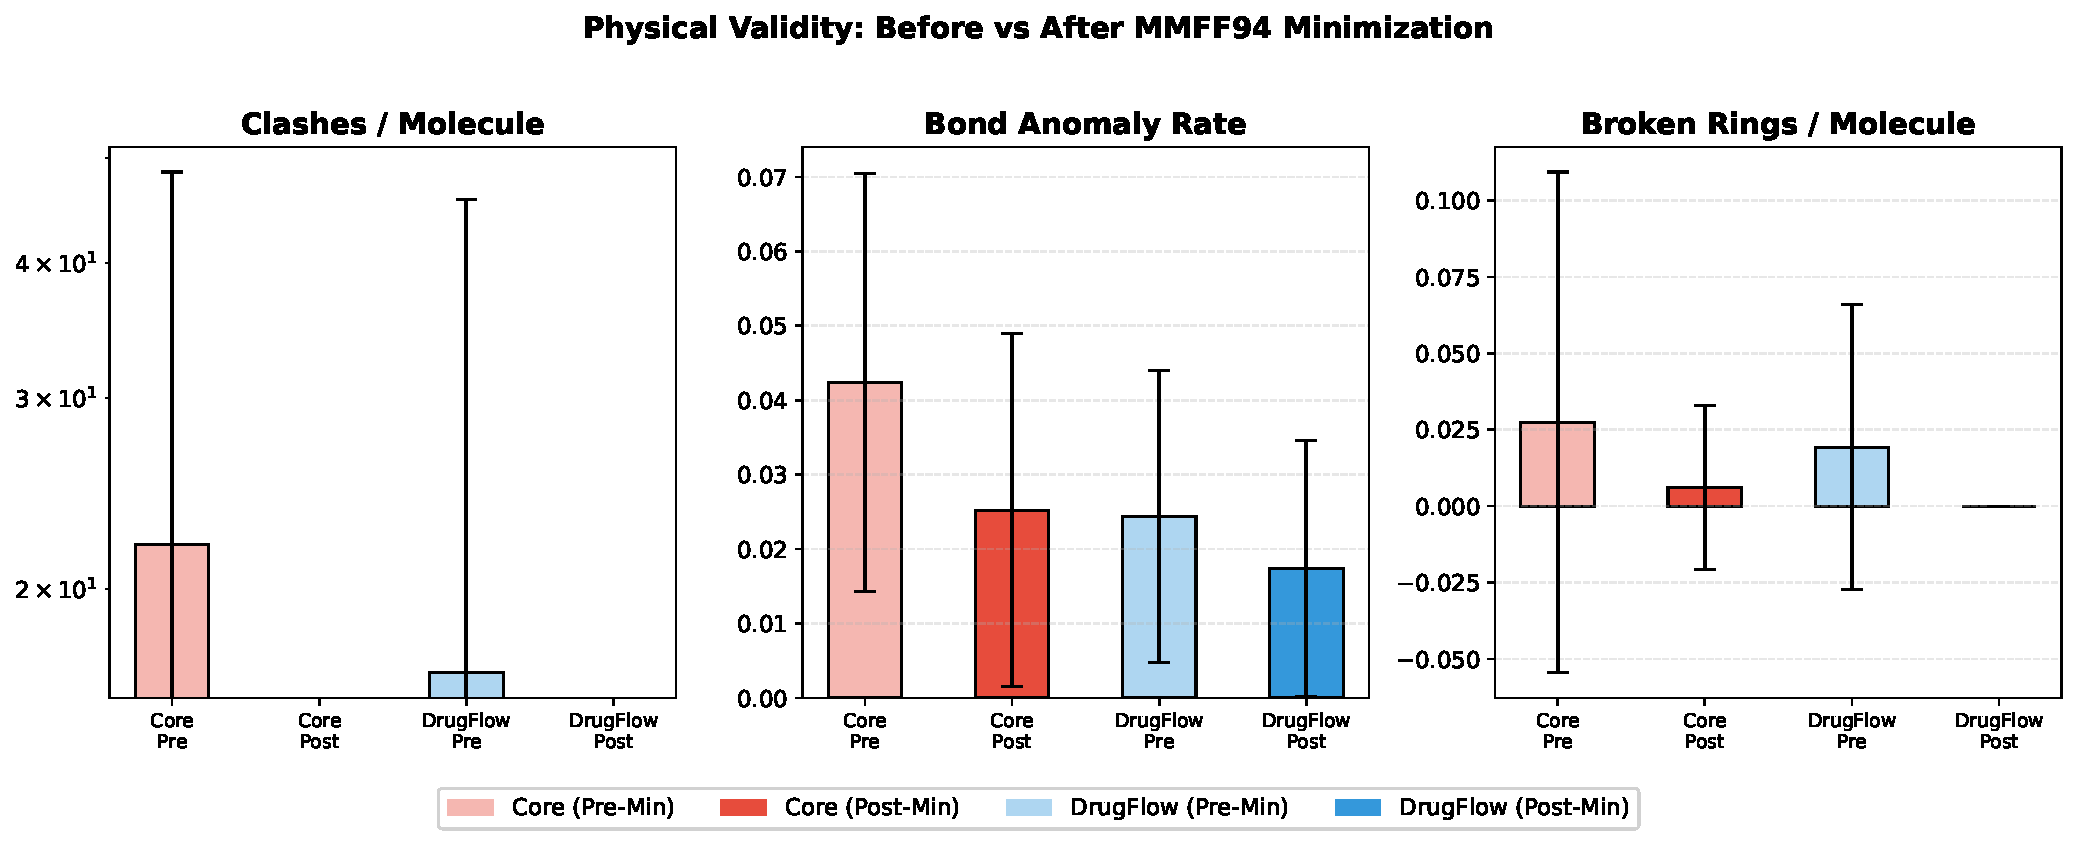
\includegraphics[width=0.78\textwidth]{output/figures/fig4.pdf}
  \caption{\textbf{Physical validity before and after MMFF94 minimization.}
    Both SV-Flow Core and DrugFlow show substantial improvement after
    minimization: steric clashes are eliminated (0.00 clashes/mol), bond
    anomalies are reduced, and broken rings are largely resolved.}
  \label{fig:physical}
\end{figure}

\begin{figure}[H]
  \centering
  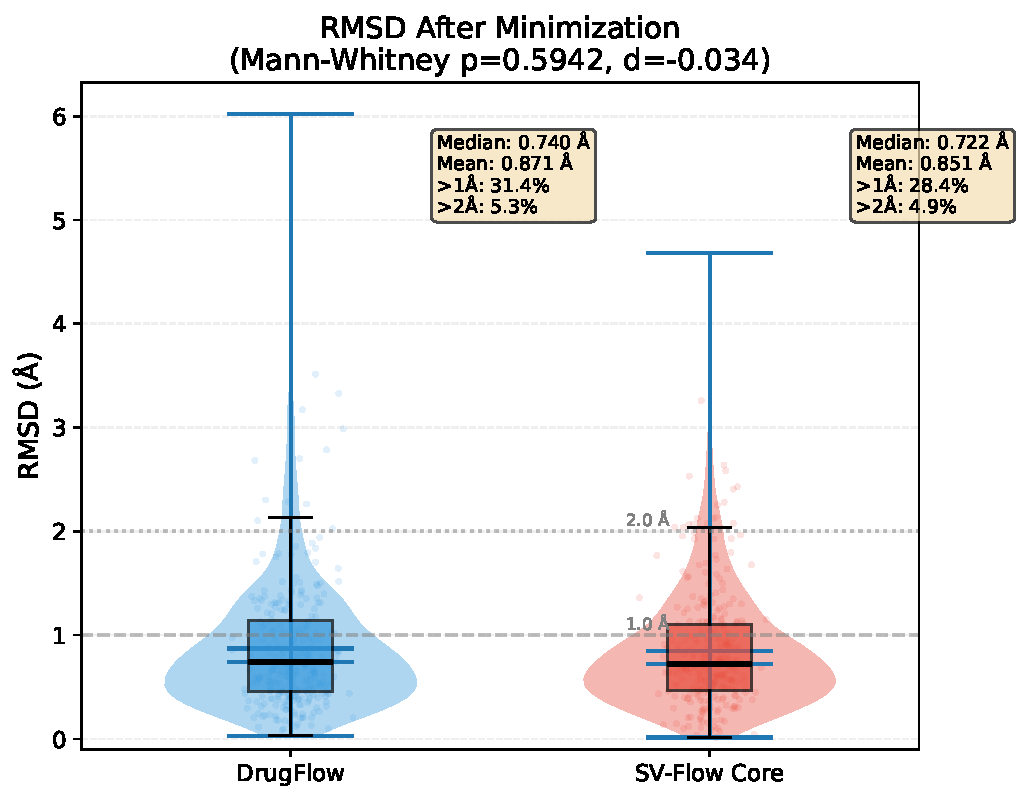
\includegraphics[width=0.78\textwidth]{output/figures/fig5.pdf}
  \caption{\textbf{RMSD distribution after MMFF94 minimization.}
    Median RMSD $<$ 0.8\,\AA\ for both methods, with $<$5\% of molecules
    exceeding 2.0\,\AA, confirming that minimization produces only minor
    conformational adjustments and does not distort the generated structures.}
  \label{fig:rmsd}
\end{figure}

\subsection{Computational Cost Breakdown}

\begin{table}[H]
\centering
\caption{Per-variant computational cost (5 pockets $\times$ 10 trajectories,
         $T = 500$ steps, NVIDIA RTX 4090 D).}
\label{tab:cost}
\begin{tabular}{l c c c}
\toprule
\textbf{Variant} & \textbf{Total Time (s)} & \textbf{Molecules/s} & \textbf{GPU Memory (GB)} \\
\midrule
Core          & 108 & 0.46 & $\sim$2.2 \\
FULL (TP+OP)  & 106 & 0.47 & $\sim$2.3 \\
w/o OP        & 106 & 0.47 & $\sim$2.3 \\
w/o TP        & 106 & 0.47 & $\sim$2.2 \\
Isotropic     & 106 & 0.47 & $\sim$2.2 \\
\bottomrule
\end{tabular}
\end{table}

The SVGD repulsion accounts for approximately 22\% of total runtime
($\sim$23 s / 106 s), consistent with the expected $O(N^2 \cdot 3)$ complexity.
The base model forward pass dominates runtime ($\sim$80\%), confirming that the
guidance overhead is modest.

\section{Case Studies}

\begin{figure}[H]
  \centering
  \textbf{Highest diversity gain}: Pocket achieving the largest
    $\Delta$Tanimoto (Core $-$ DrugFlow).  Colored sticks: SV-Flow Core
    molecules.  Gray sticks: DrugFlow baseline molecules.  SV-Flow molecules
    explore more diverse spatial positions and chemical scaffolds.
  \label{fig:case_high}
\end{figure}

\begin{figure}[H]
  \centering
  \textbf{Lowest diversity gain}: Pocket achieving the smallest
    $\Delta$Tanimoto.  In geometrically constrained pockets, even SV-Flow
    molecules cluster similarly to DrugFlow, indicating that pocket geometry can
    limit the achievable diversity.
  \label{fig:case_low}
\end{figure}

\begin{figure}[H]
  \centering
  \textbf{Median diversity gain}: A representative pocket showing the typical
    behavior of SV-Flow relative to DrugFlow.
  \label{fig:case_median}
\end{figure}

\noindent\textit{Note}: Interactive 3D visualizations of these case studies are
available as HTML files in \texttt{output/figures/fig6\_*.html}.

\end{document}
